\subsubsection*{21.7}

Запишем лагранжиан системы
\begin{equation*}
    L = T - \Pi = \frac{1}{2} m \dot{x}^2 + \frac{1}{2} m x^2 \omega^2.
\end{equation*}
В условиях сказано, что $\omega = \omega(t)$ -- для простоты уравнений будем считать $\omega = \const$.

\begin{figure}[h]
    \centering
    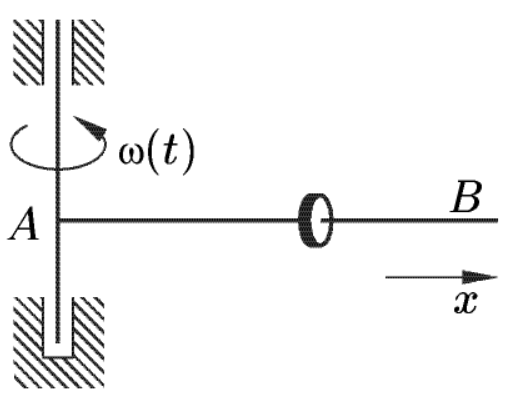
\includegraphics[width=0.25\textwidth]{figures/21.7.png}
    \caption{К задаче 21.7}
    %\label{fig:}
\end{figure}

Действие тогда
\begin{equation*}
    S = \int_{t_1}^{t_2} L \d t,
    \hspace{0.5cm} \Rightarrow \hspace{0.5cm} 
    \delta S = m
        \dot{x} \delta x \bigg|_{t_1}^{t_2}
        +
        m\int_0^t
        \left(
        - \ddot{x} + x \omega^2
        \right) \delta x \d t
     = 0.
\end{equation*}
Так приходим к
\begin{equation*}
    \ddot{x} = \omega^2 (t) x,
    \hspace{0.5cm} \Rightarrow \hspace{0.5cm} 
    x = A e^{\omega t} + B e^{-\omega t}.
\end{equation*}
Рассмотрим движение от $(x_1, t_1)$ до $(x_2, t_2)$, получим СЛУ:
\begin{equation*}
    \left\{\begin{aligned}
        x_1 &= A e^{\omega t_1} + B e^{-\omega t_1} \\
        x_2 &= A e^{\omega t_2} + B e^{-\omega t_2}
    \end{aligned}\right.
    \hspace{0.5cm} \Rightarrow \hspace{0.5cm} 
    \det = e^{\omega(t_1 - t_2)} - e^{-\omega(t_1 - t_2)} \neq 0,
     \hspace{0.25cm} \text{ при } t \neq \const,
\end{equation*}
что соответствует существованию единственного решения у уравнения.